\documentclass[12pt,a4paper]{article}
\usepackage[utf8]{inputenc}
\usepackage[T1]{fontenc}
\usepackage[english]{babel}
\graphicspath{{./figs/}}
\usepackage{amsmath,amssymb}
\usepackage{graphicx}
\usepackage{booktabs}
\usepackage{array}
\usepackage{longtable}
\usepackage{float}
\usepackage{listings}
\usepackage{xcolor}
\usepackage{hyperref}
\usepackage[left=2.5cm,right=2.5cm,top=2.5cm,bottom=2.5cm]{geometry}
\usepackage{caption}
\usepackage{subcaption}

\lstdefinestyle{pythonstyle}{
    language=Python,
    basicstyle=\ttfamily\small,
    keywordstyle=\color{blue}\bfseries,
    stringstyle=\color{red},
    commentstyle=\color{gray}\itshape,
    numbers=left,
    numberstyle=\tiny\color{gray},
    stepnumber=1,
    numbersep=5pt,
    backgroundcolor=\color{gray!5},
    frame=single,
    rulecolor=\color{gray!30},
    breaklines=true,
    showstringspaces=false,
    tabsize=4,
    captionpos=b
}
\lstset{style=pythonstyle}

\begin{document}

%% =============================================================
%% CHAPTER X — PREPROCESSING & MODEL IMPLEMENTATION
%% =============================================================

\section{Data Preprocessing and Detection Models Implementation}

\subsection{Introduction}

In the context of the \textbf{AEGIS Entropy} project, the artificial intelligence-based detection module constitutes the core component of the defense system against \textit{Port Scan} attacks. This phase of the project aims to design, implement, and evaluate a comprehensive Machine Learning pipeline, strictly adhering to the PDCA (\textit{Plan-Do-Check-Act}) methodology and the academic standards taught in class.

The primary objective is to build a detection pipeline capable of achieving the success criteria defined in the project's final plan:
\begin{itemize}
    \item \textbf{F1-Score} $\geq$ 88\%
    \item \textbf{Accuracy} $\geq$ 90\%
    \item \textbf{False Positive Rate (FPR)} $<$ 6\%
\end{itemize}

This chapter details every step of the pipeline: from exploring and cleaning the raw data, through selecting features according to the Data Dictionary, to the training, cross-validation, and final evaluation of the three selected models: \textbf{Random Forest}, \textbf{XGBoost}, and \textbf{Isolation Forest}.

%% =============================================================
\subsection{Dataset Used}

The dataset used for training and evaluating the models is \textbf{CICIDS2017} (\textit{Canadian Institute for Cybersecurity Intrusion Detection System}), an academic benchmark dataset for network intrusion detection. It was generated in a controlled environment replicating realistic network traffic conditions, including both benign traffic and simulated attacks.

The specific file utilized is:
\begin{center}
\texttt{Friday-WorkingHours-Afternoon-PortScan.pcap\_ISCX.csv}
\end{center}

\noindent This file contains network flows captured on Friday afternoon, a period during which \textit{Port Scan} attacks (via \texttt{Nmap}) were executed.

\begin{table}[H]
\centering
\caption{Dataset characteristics}
\begin{tabular}{ll}
\toprule
\textbf{Property} & \textbf{Value} \\
\midrule
Number of instances (rows) & 286,467 \\
Number of features (columns) & 79 \\
\texttt{PortScan} class & 158,930 (55.48\%) \\
\texttt{BENIGN} class & 127,537 (44.52\%) \\
Format & CSV (aggregated network flows) \\
\bottomrule
\end{tabular}
\end{table}

\noindent A slight imbalance in favor of the \texttt{PortScan} class is observed, which will be addressed later using the SMOTE technique (Section~\ref{sec:smote}).

\begin{figure}[H]
\centering
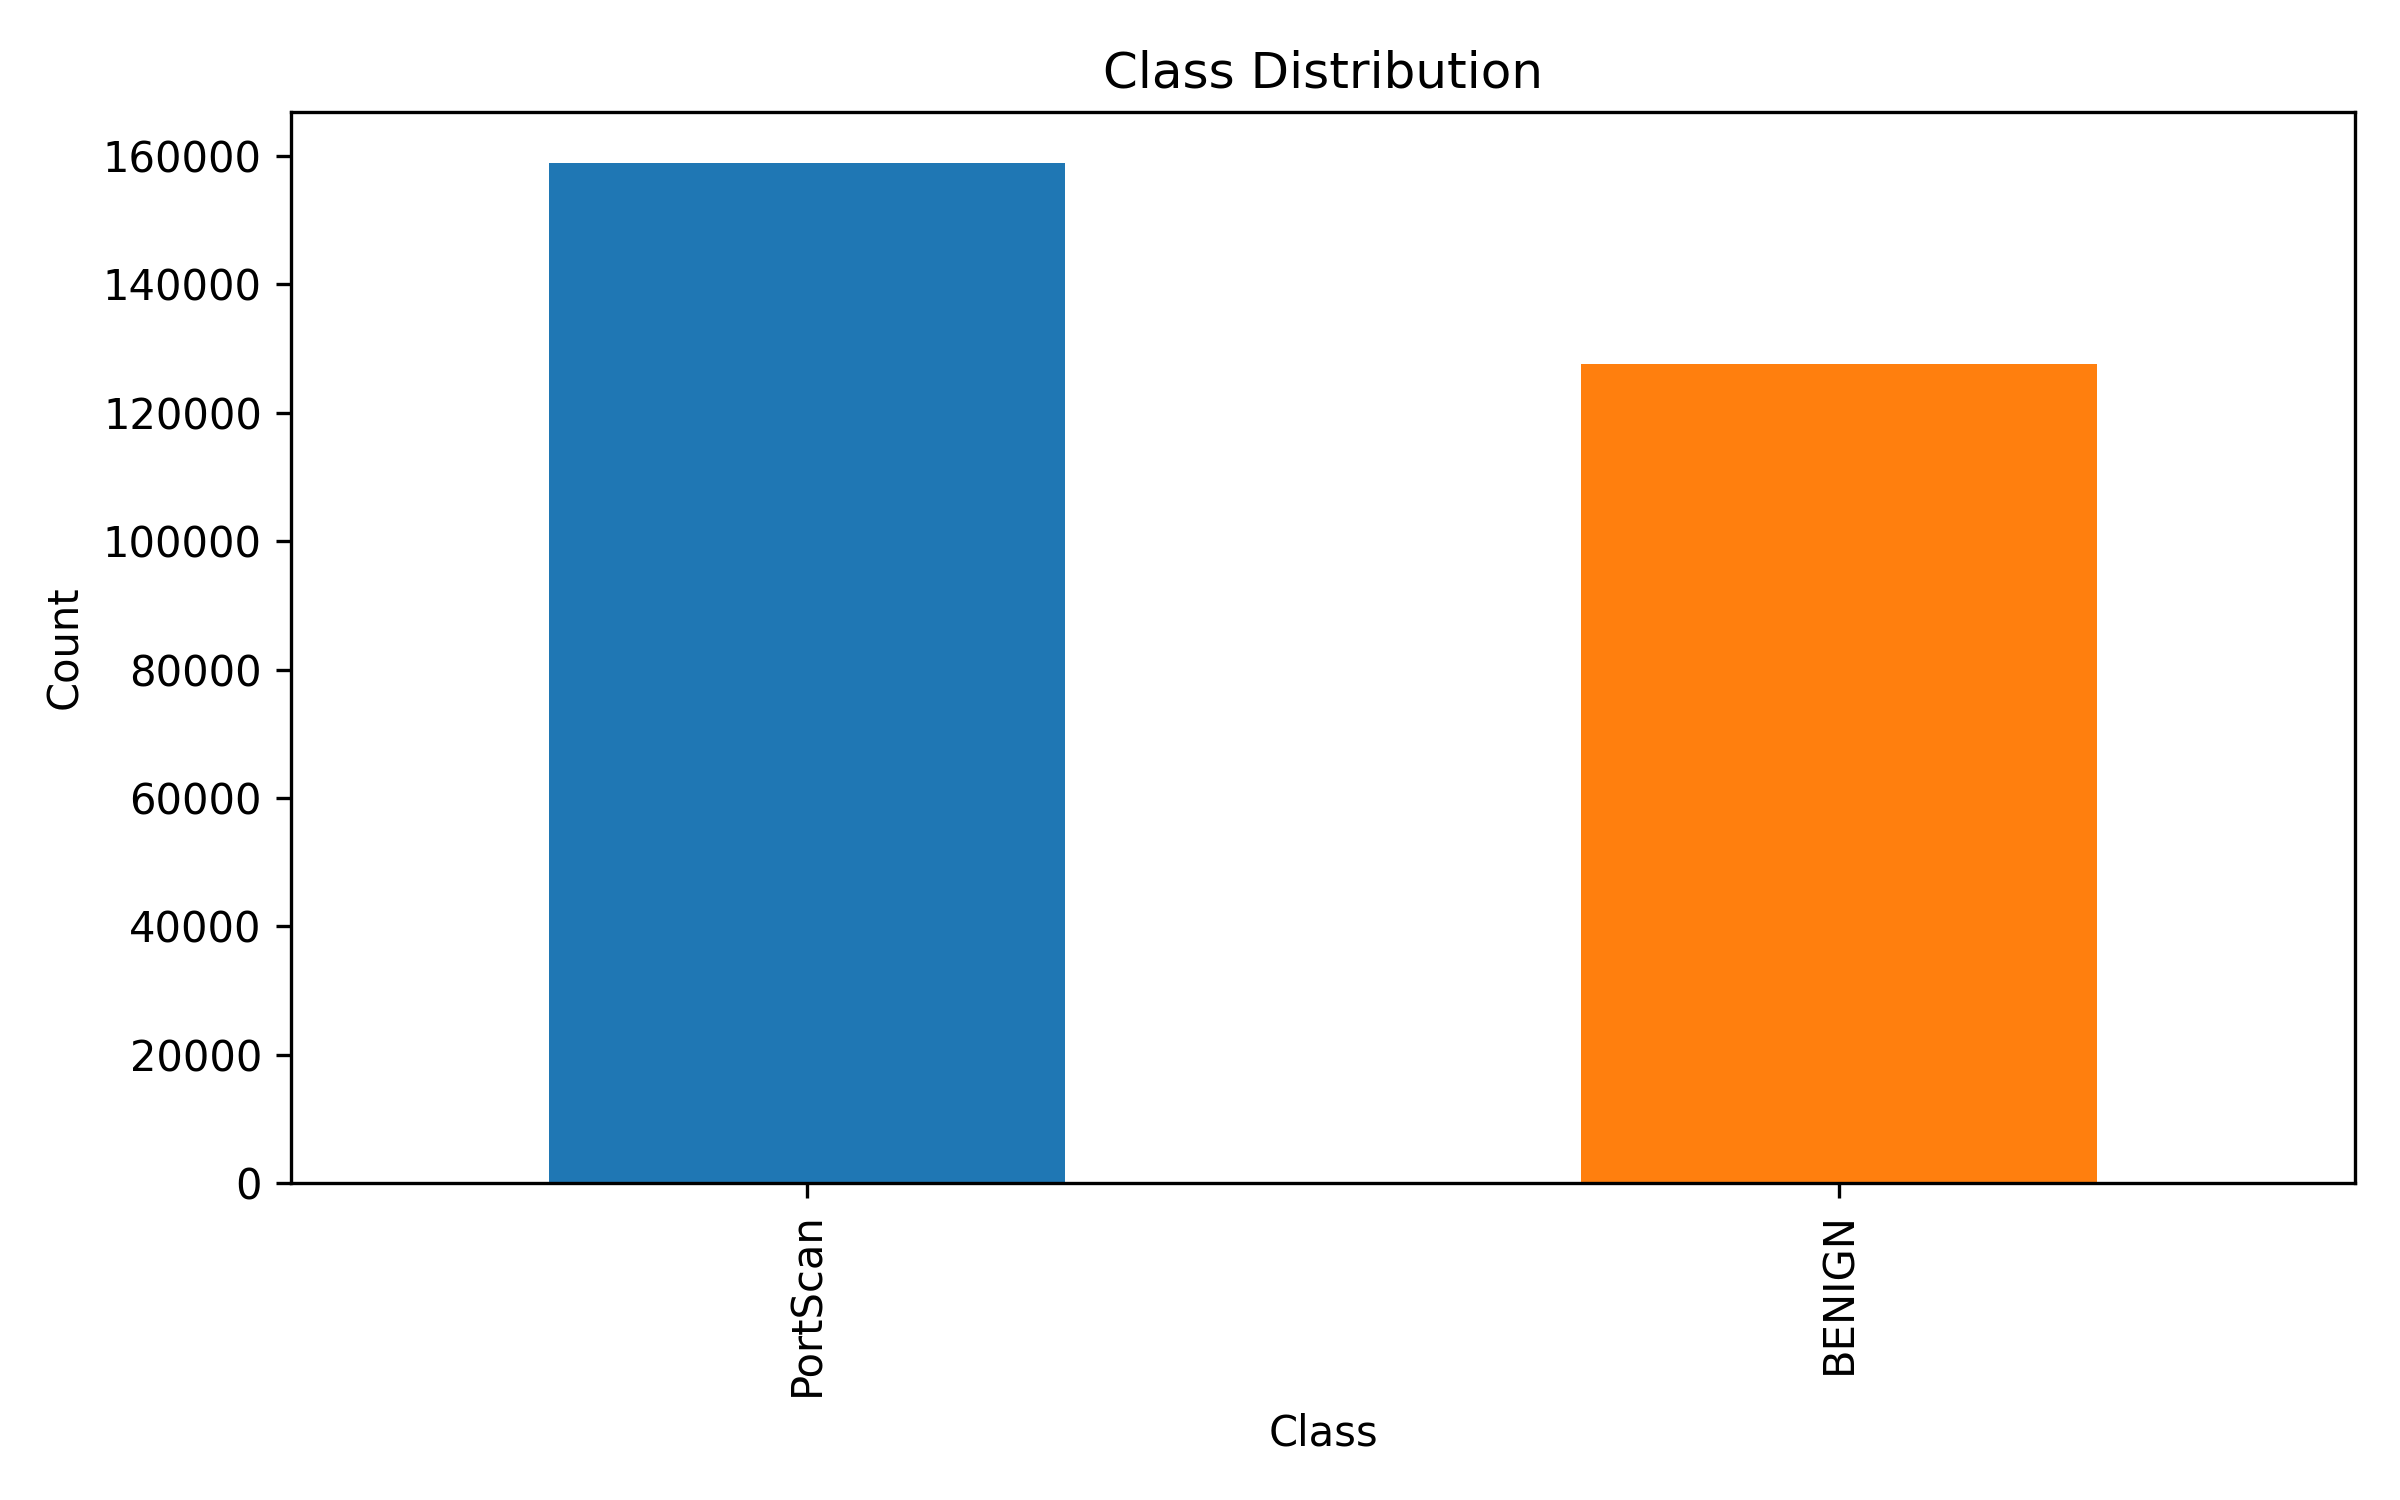
\includegraphics[width=0.72\textwidth]{class_distribution.png}
\caption{Class distribution in the CICIDS2017 dataset (PortScan vs BENIGN)}
\label{fig:class_dist}
\end{figure}

%% =============================================================
\subsection{Feature Selection (Data Dictionary)}

The project's Data Dictionary defines \textbf{13 features} deemed relevant for detecting Port Scan attacks. However, since the CICIDS2017 dataset is a collection of aggregated flow data (\textit{flow-level}), it does not directly contain all these features. A \textbf{mapping} process was conducted to establish the correspondence between the theoretical features and the available CSV columns.

\begin{longtable}{p{3.8cm}cp{3.5cm}p{4cm}}
\caption{Feature Mapping: Data Dictionary $\rightarrow$ CSV Columns} \label{tab:feature_mapping} \\
\toprule
\textbf{Feature (Dict.)} & \textbf{Avail.} & \textbf{CSV Column} & \textbf{Justification} \\
\midrule
\endfirsthead
\toprule
\textbf{Feature (Dict.)} & \textbf{Avail.} & \textbf{CSV Column} & \textbf{Justification} \\
\midrule
\endhead
Distinct Dst Ports & $\approx$ & Destination Port & Proxy: the variance of ports targeted by scanners provides a discriminative signal \\
SYN Flag Count & \checkmark & SYN Flag Count & Direct match \\
RST Flag Count & \checkmark & RST Flag Count & Direct match \\
Flow Duration & \checkmark & Flow Duration & Direct match \\
Total Fwd Packets & \checkmark & Total Fwd Packets & Direct match \\
ACK Flag Count & \checkmark & ACK Flag Count & Direct match \\
IAT Mean & \checkmark & Flow IAT Mean & Direct match \\
Bwd Packet Length & \checkmark & Bwd Packet Length Mean & Mean variant \\
TCP Window Size & \checkmark & Init\_Win\_bytes\_forward & Best proxy available in CICIDS2017 \\
\midrule
Unique Dst IPs & $\times$ & --- & Absent from CSV; live capture feature only \\
TTL Value & $\times$ & --- & Absent from flow-level data \\
Shadow Node Interaction & N/A & Placeholder = 0 & Future integration with honeypot module \\
MTD Port Delta & N/A & Placeholder = 0 & Future integration with MTD module \\
\bottomrule
\end{longtable}

\noindent \textbf{Final Decision:} The pipeline uses \textbf{11 features} in total: 9 extracted from the CSV + 2 placeholders (initialized to 0) reserved for real-time integration with the honeypot and MTD modules.

\begin{lstlisting}[caption={Defining features in the pipeline},label={lst:features}]
features = [
    'Destination Port',        # Proxy for Distinct Dst Ports
    'Flow Duration',
    'Total Fwd Packets',
    'SYN Flag Count',
    'RST Flag Count',
    'ACK Flag Count',
    'Flow IAT Mean',
    'Bwd Packet Length Mean',
    'Init_Win_bytes_forward'   # Proxy for TCP Window Size
]
X = df[features].copy()
X['shadow_node_interaction'] = 0  # Honeypot placeholder
X['mtd_port_delta'] = 0           # MTD placeholder
\end{lstlisting}

\begin{figure}[H]
\centering
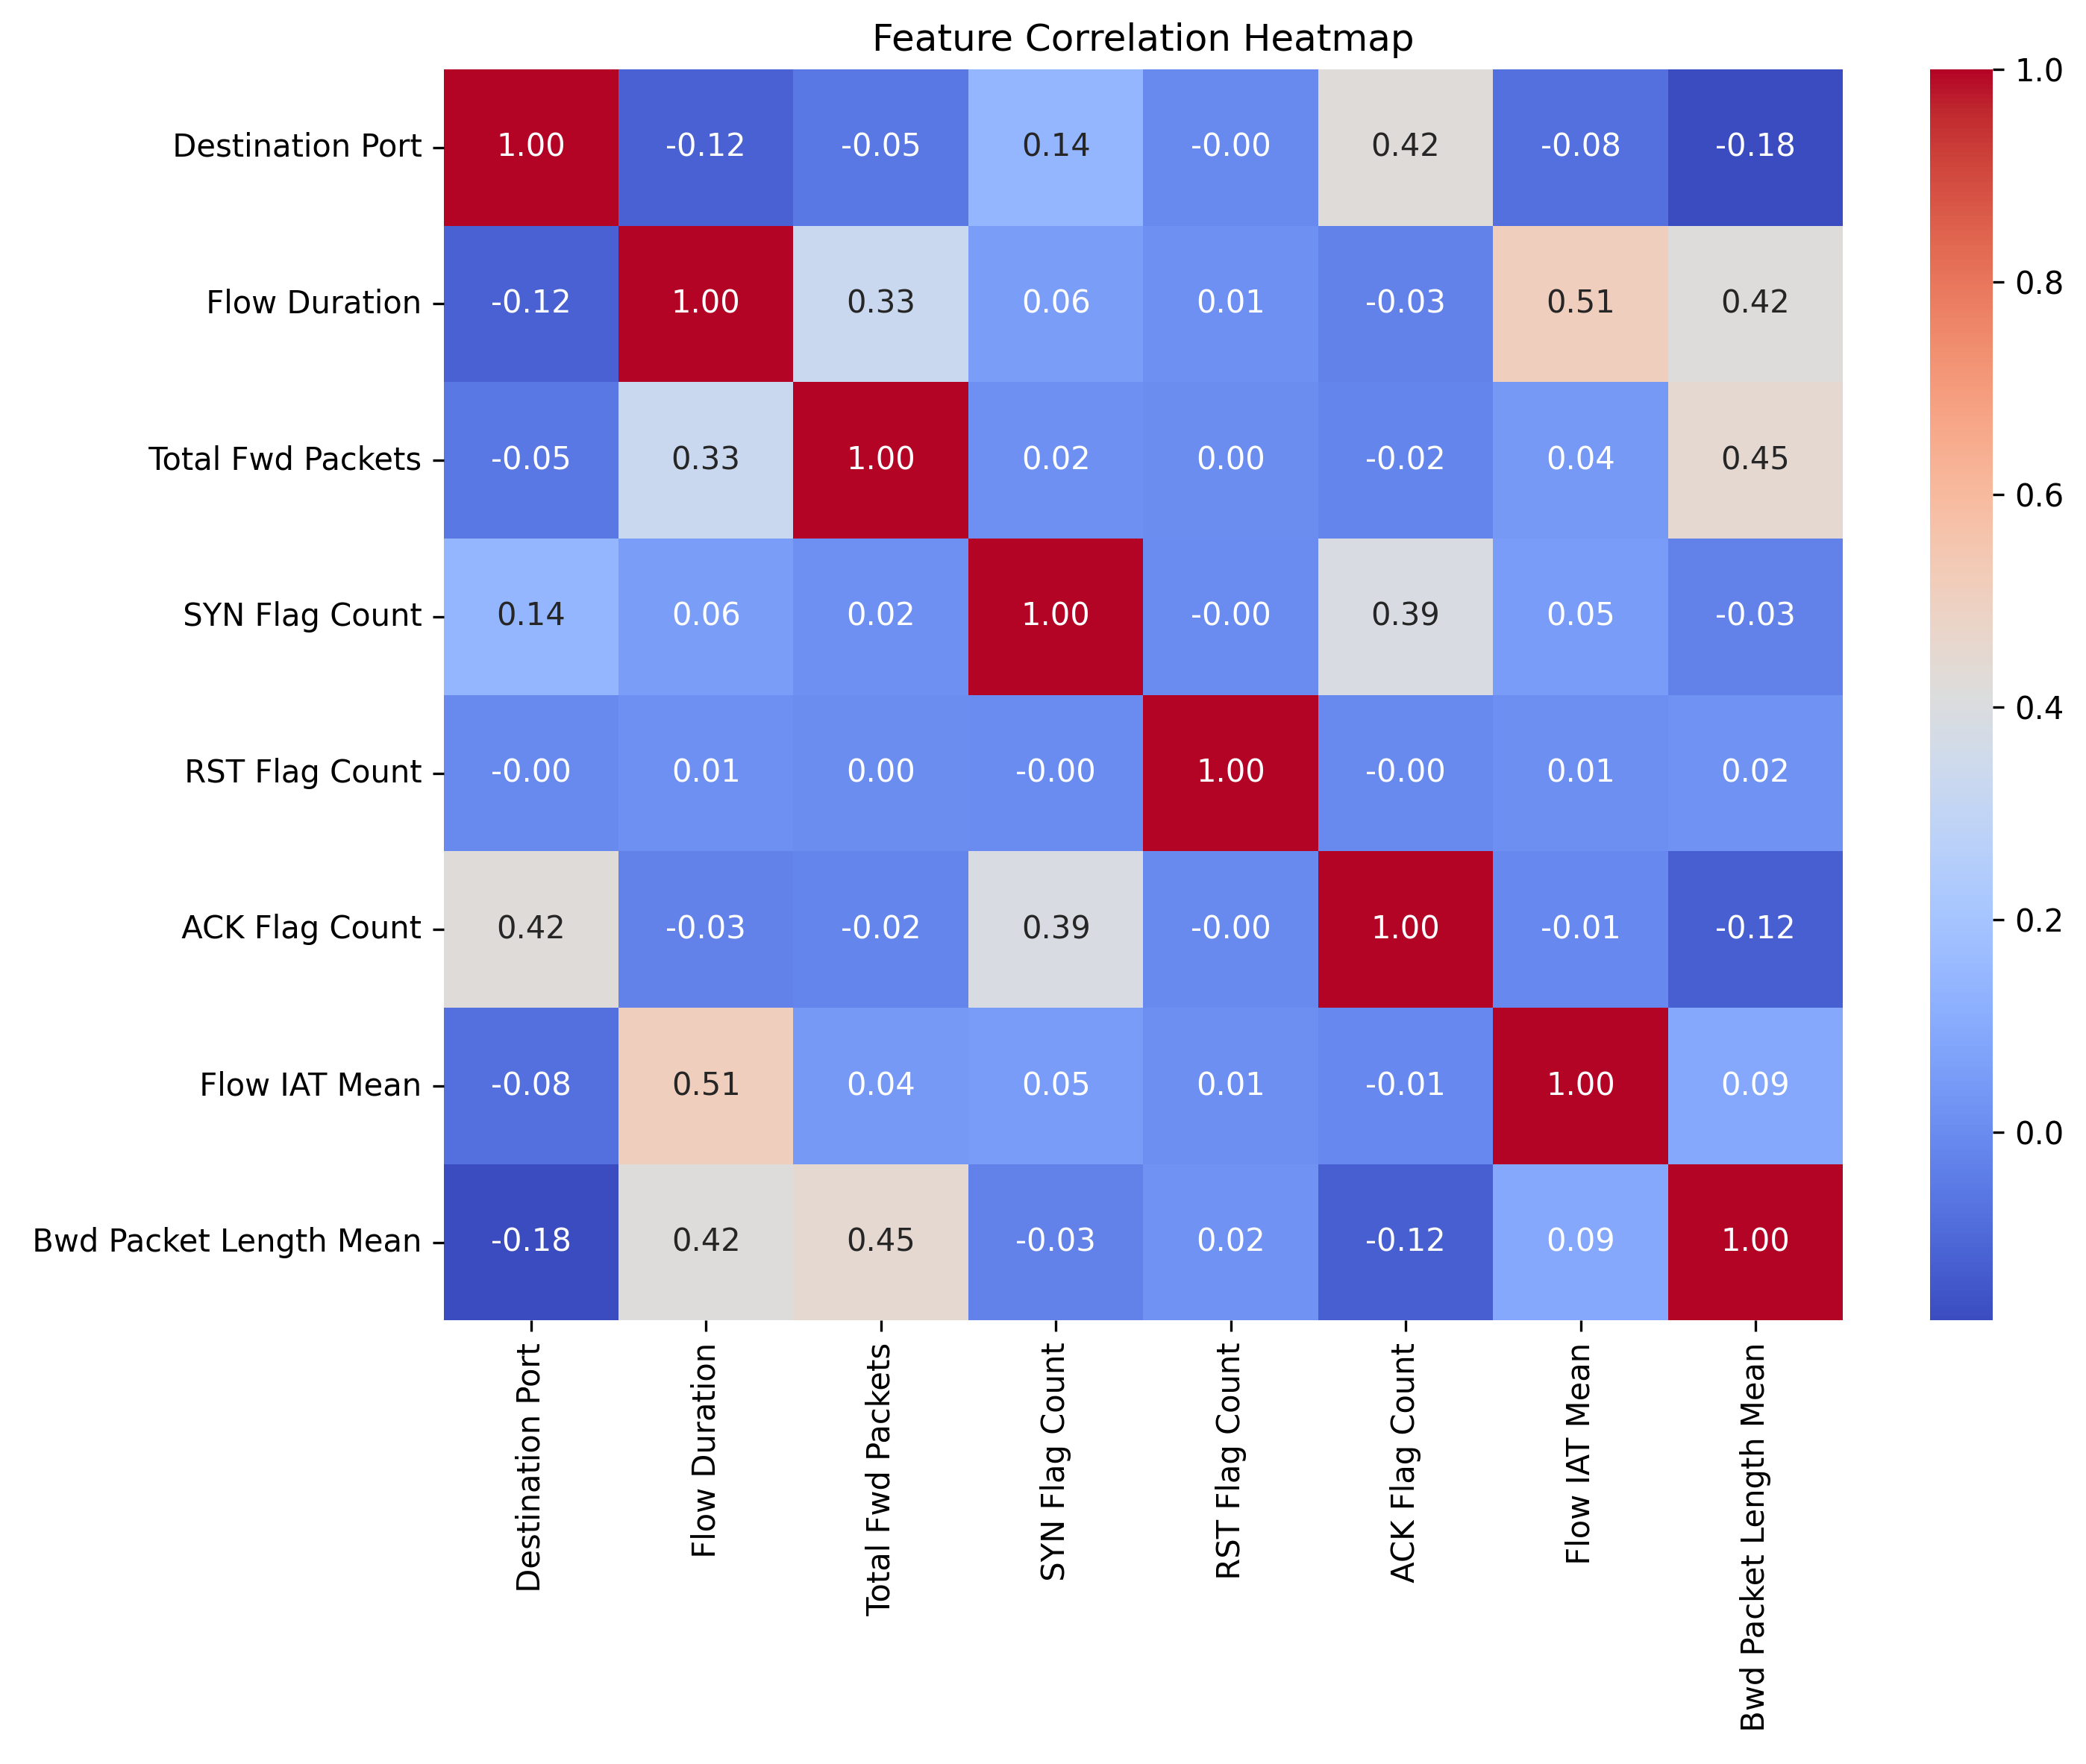
\includegraphics[width=0.88\textwidth]{correlation_heatmap.png}
\caption{Correlation matrix between selected features}
\label{fig:corr_heatmap}
\end{figure}

%% =============================================================
\subsection{Preprocessing Pipeline}

Data preprocessing is a critical step that directly influences model quality. Following the methodology taught in class, the pipeline follows a sequential four-step process: cleaning, outlier detection, skewness correction, and export.

\subsubsection{Data Cleaning}

The first step involves preparing the raw data for analysis. The CICIDS2017 dataset presents several common issues:

\begin{enumerate}
    \item \textbf{Spaces in column names:} CSV headers contain leading spaces (e.g., \texttt{' Flow Duration'} instead of \texttt{'Flow Duration'}). These spaces cause silent errors when accessing columns.
    \item \textbf{Infinite values:} Some columns contain \texttt{inf} or \texttt{-inf} values, resulting from division by zero during network flow calculations.
    \item \textbf{Missing values:} After replacing infinities, \texttt{NaN} values may remain.
\end{enumerate}

\begin{lstlisting}[caption={Cleaning raw data}]
# 1. Remove spaces in column names
df.columns = [col.strip() for col in df.columns]

# 2. Replace infinite values with NaN
df.replace([np.inf, -np.inf], np.nan, inplace=True)

# 3. Imputation by median (robust to outliers)
df[FEATURES] = df[FEATURES].fillna(df[FEATURES].median())
\end{lstlisting}

\noindent \textbf{Choice of median:} Unlike the mean (sensitive to extreme values) or zero replacement (which introduces bias), the median provides a robust estimation of central tendency, particularly suited for the asymmetric distributions typical of network traffic.

\subsubsection{Outlier Detection and Handling (IQR Method)}

Outliers can distort model training by creating biases in distributions. The \textbf{Interquartile Range (IQR)} method is used to detect them in a statistically rigorous manner.

\paragraph{Formal Definition:} Let $Q_1$ be the first quartile (25\textsuperscript{th} percentile) and $Q_3$ be the third quartile (75\textsuperscript{th} percentile) of a variable. The interquartile range is defined by:
\begin{equation}
    IQR = Q_3 - Q_1
\end{equation}

\noindent The detection bounds are:
\begin{equation}
    \text{Lower Bound} = Q_1 - 1.5 \times IQR \qquad ; \qquad \text{Upper Bound} = Q_3 + 1.5 \times IQR
\end{equation}

\noindent Any observation outside the interval $[\text{Lower Bound},\; \text{Upper Bound}]$ is considered an outlier.

\paragraph{Handling Strategy:} Rather than \textbf{removing} rows containing outliers (which risks losing valuable attack data), we apply \textbf{capping} (\textit{Winsorization}): values beyond the bounds are adjusted to the nearest bound.

\begin{lstlisting}[caption={Outlier detection and capping using IQR}]
for feature in FEATURES:
    Q1 = df[feature].quantile(0.25)
    Q3 = df[feature].quantile(0.75)
    IQR = Q3 - Q1
    lower_bound = Q1 - 1.5 * IQR
    upper_bound = Q3 + 1.5 * IQR

    # Count detected outliers
    outliers = ((df[feature] < lower_bound) |
                (df[feature] > upper_bound)).sum()

    # Capping instead of removal
    df[feature] = np.where(
        df[feature] < lower_bound, lower_bound, df[feature])
    df[feature] = np.where(
        df[feature] > upper_bound, upper_bound, df[feature])
\end{lstlisting}

\begin{table}[H]
\centering
\caption{Number of outliers detected per feature (IQR method)}
\label{tab:outliers}
\begin{tabular}{lr}
\toprule
\textbf{Feature} & \textbf{Detected Outliers} \\
\midrule
Destination Port & 37,788 \\
Flow Duration & 52,212 \\
Total Fwd Packets & 35,156 \\
SYN Flag Count & 6,014 \\
RST Flag Count & 21 \\
ACK Flag Count & 35,555 \\
Flow IAT Mean & 57,303 \\
Bwd Packet Length Mean & 32,387 \\
Init\_Win\_bytes\_forward & 0 \\
\bottomrule
\end{tabular}
\end{table}

\begin{figure}[H]
\centering
\begin{subfigure}[b]{0.32\textwidth}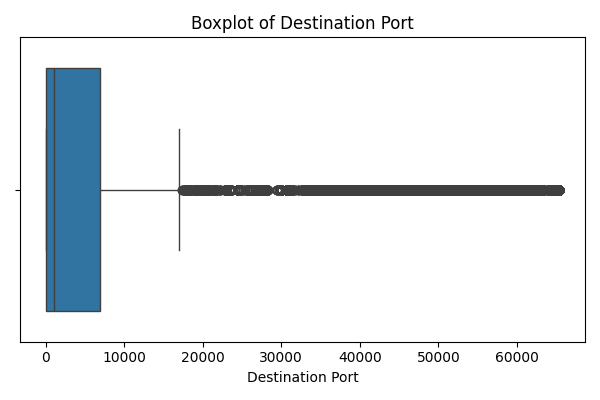
\includegraphics[width=\textwidth]{boxplot_Destination_Port.png}\caption{Destination Port}\end{subfigure}\hfill
\begin{subfigure}[b]{0.32\textwidth}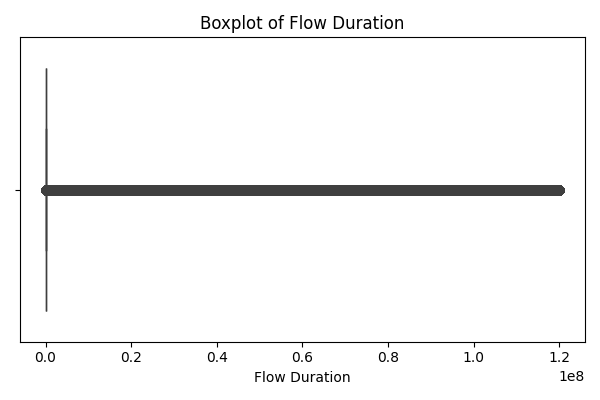
\includegraphics[width=\textwidth]{boxplot_Flow_Duration.png}\caption{Flow Duration}\end{subfigure}\hfill
\begin{subfigure}[b]{0.32\textwidth}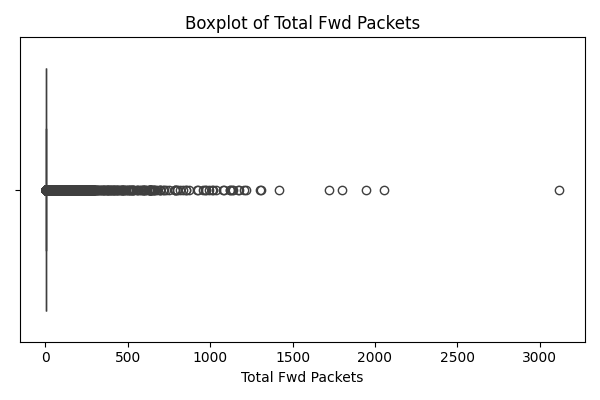
\includegraphics[width=\textwidth]{boxplot_Total_Fwd_Packets.png}\caption{Total Fwd Packets}\end{subfigure}
\vspace{0.5em}
\begin{subfigure}[b]{0.32\textwidth}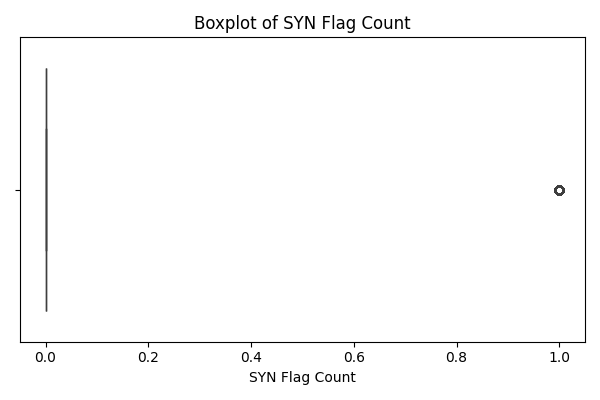
\includegraphics[width=\textwidth]{boxplot_SYN_Flag_Count.png}\caption{SYN Flag Count}\end{subfigure}\hfill
\begin{subfigure}[b]{0.32\textwidth}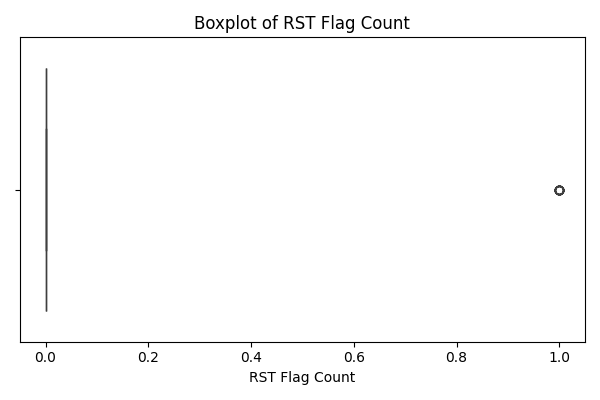
\includegraphics[width=\textwidth]{boxplot_RST_Flag_Count.png}\caption{RST Flag Count}\end{subfigure}\hfill
\begin{subfigure}[b]{0.32\textwidth}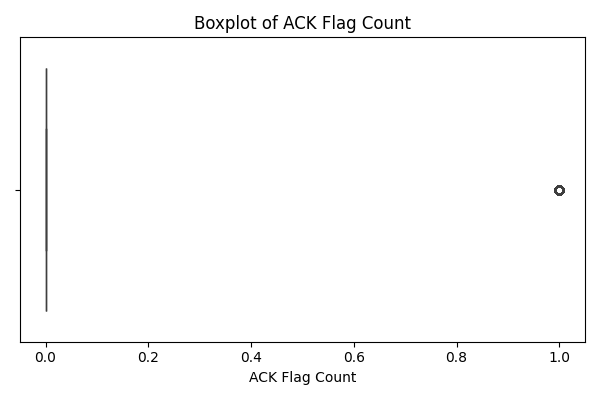
\includegraphics[width=\textwidth]{boxplot_ACK_Flag_Count.png}\caption{ACK Flag Count}\end{subfigure}
\vspace{0.5em}
\begin{subfigure}[b]{0.32\textwidth}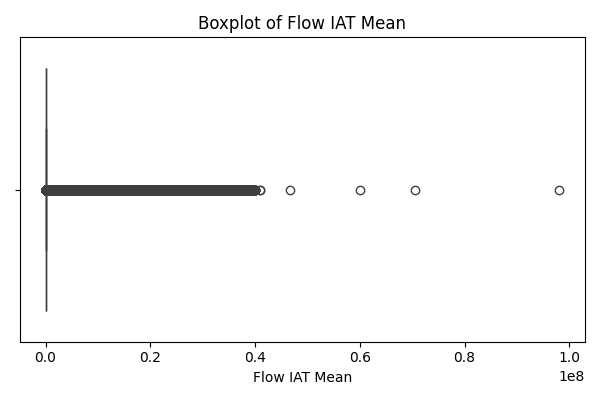
\includegraphics[width=\textwidth]{boxplot_Flow_IAT_Mean.png}\caption{Flow IAT Mean}\end{subfigure}\hfill
\begin{subfigure}[b]{0.32\textwidth}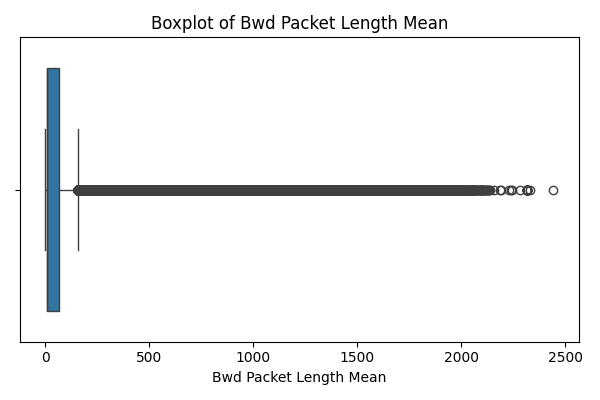
\includegraphics[width=\textwidth]{boxplot_Bwd_Packet_Length_Mean.png}\caption{Bwd Pkt Length Mean}\end{subfigure}\hfill
\begin{subfigure}[b]{0.32\textwidth}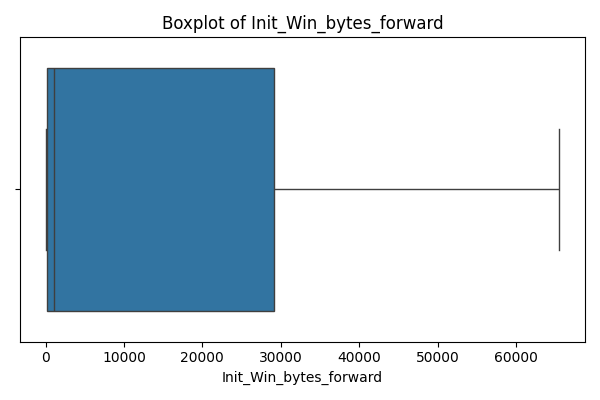
\includegraphics[width=\textwidth]{boxplot_Init_Win_bytes_forward.png}\caption{Init Win Bytes Fwd}\end{subfigure}
\caption{Boxplots of all 9 selected features illustrating the presence and extent of outliers}
\label{fig:boxplots}
\end{figure}

\subsubsection{Skewness Analysis and Logarithmic Transformation}

Skewness measures the degree of asymmetry of a distribution relative to a normal distribution. Fisher's coefficient is defined by:
\begin{equation}
    \gamma_1 = \frac{E[(X - \mu)^3]}{\sigma^3}
\end{equation}

\noindent where $\mu$ is the mean and $\sigma$ the standard deviation. A value of $|\gamma_1| > 1$ indicates strong skewness, justifying a transformation to normalize the distribution.

\paragraph{Applied Transformation:} For features exhibiting strong skewness ($|\text{skew}| > 1.0$), we apply the logarithmic transformation $\log(1 + x)$ (function \texttt{np.log1p}). Using $\log(1+x)$ rather than $\log(x)$ is essential because it:
\begin{itemize}
    \item Properly handles zero values ($\log(1+0) = 0$)
    \item Preserves the relative order of observations
    \item Reduces the influence of extreme values on the distribution
\end{itemize}

\begin{lstlisting}[caption={Skewness analysis and logarithmic transformation}]
for feature in FEATURES:
    skewness = df[feature].skew()
    if abs(skewness) > 1.0:
        # Shift if negative values exist
        min_val = df[feature].min()
        if min_val < 0:
            df[feature] = df[feature] - min_val
        # Log(1+x) transformation
        df[feature] = np.log1p(df[feature])
\end{lstlisting}

\begin{table}[H]
\centering
\caption{Feature skewness analysis}
\label{tab:skewness}
\begin{tabular}{lrl}
\toprule
\textbf{Feature} & \textbf{Skewness} & \textbf{Action} \\
\midrule
Destination Port & 1.29 & Log transform applied \\
Flow Duration & 1.27 & Log transform applied \\
Total Fwd Packets & 1.32 & Log transform applied \\
SYN Flag Count & 0.00 & None \\
RST Flag Count & 0.00 & None \\
ACK Flag Count & 0.00 & None \\
Flow IAT Mean & 1.24 & Log transform applied \\
Bwd Packet Length Mean & 1.27 & Log transform applied \\
Init\_Win\_bytes\_forward & 0.96 & None ($< 1.0$) \\
\bottomrule
\end{tabular}
\end{table}

\subsubsection{Preprocessed Dataset Export}

After all transformations, the cleaned dataset is exported in CSV format to ensure the \textbf{reproducibility} of the pipeline. The training and evaluation scripts directly consume this preprocessed file.

\begin{lstlisting}[caption={Preprocessed dataset export}]
df.to_csv("../data/preprocessed.csv", index=False)
\end{lstlisting}

%% =============================================================
\subsection{Data Splitting and Normalization}

\subsubsection{Train/Test Split (80/20)}

The preprocessed dataset is divided into a training set (80\%) and a test set (20\%), using \textbf{stratified sampling} to preserve class proportions in each partition.

\begin{lstlisting}[caption={Stratified dataset splitting}]
X_train, X_test, y_train, y_test = train_test_split(
    X, y,
    test_size=0.2,
    random_state=42,    # Reproducibility
    stratify=y          # Preserves class proportions
)
# Result: Train = 229,173 | Test = 57,294
\end{lstlisting}

\subsubsection{Standardization (StandardScaler)}
\label{sec:standardscaler}

Standardization transforms each feature to have a mean of 0 and a standard deviation of 1, according to the formula:
\begin{equation}
    z = \frac{x - \mu}{\sigma}
\end{equation}

\noindent where $\mu$ and $\sigma$ are respectively the mean and standard deviation of the feature \textbf{calculated solely on the training set}.

\paragraph{Data Leakage Prevention:} It is imperative that the \texttt{StandardScaler} is fitted (\texttt{fit}) \textbf{exclusively on the training data}. If the scaler were fitted on the entire dataset (train + test), the test set statistics would contaminate the learning process, skewing evaluation results. The scaler is then saved to be reused during production inference.

\begin{lstlisting}[caption={Standardization with data leakage prevention}]
scaler = StandardScaler()
# fit() on train ONLY, then transform() on both
X_train_scaled = scaler.fit_transform(X_train)
X_test_scaled  = scaler.transform(X_test)

# Save for production inference
joblib.dump(scaler, "../models/scaler.pkl")
\end{lstlisting}

\subsubsection{Class Balancing (SMOTE)}
\label{sec:smote}

Although the imbalance is moderate (55/45), applying \textbf{SMOTE} (\textit{Synthetic Minority Oversampling Technique}) ensures unbiased training. SMOTE generates synthetic examples of the minority class by interpolating between existing nearby instances in the feature space.

\paragraph{SMOTE Principle:} For each instance of the minority class, SMOTE:
\begin{enumerate}
    \item Identifies its $k$ nearest neighbors (default $k=5$)
    \item Randomly selects one of these neighbors
    \item Creates a synthetic point on the line segment connecting the original instance to the selected neighbor
\end{enumerate}

\paragraph{Application on training data only:} SMOTE is applied \textbf{after} splitting and standardization, and \textbf{only} on the training set. Applying SMOTE before the split would introduce data leakage, as synthetic points generated from test data could end up in the training set.

\begin{lstlisting}[caption={Application of SMOTE on the training set}]
from imblearn.over_sampling import SMOTE

smote = SMOTE(random_state=42)
X_train_res, y_train_res = smote.fit_resample(
    X_train_scaled, y_train
)
# Before SMOTE: 229,173 samples (imbalanced)
# After SMOTE: 254,288 samples (balanced)
\end{lstlisting}

%% =============================================================
%% PART 2 — Sections X.6 to X.9
%% Paste this content BEFORE \end{document} in ml_pipeline_report.tex
%% =============================================================

\subsection{Model Implementation}

Three models were selected in accordance with the project's final plan, each providing a complementary approach to detection:

\subsubsection{Random Forest}

\textbf{Random Forest} is a supervised learning algorithm based on the \textit{bagging} (\textit{Bootstrap Aggregating}) principle. It builds an ensemble of $n$ decision trees, each trained on a random sub-sample of the data with a random subset of features. The final prediction is obtained by \textbf{majority vote}.

\paragraph{Advantages for Port Scan detection:}
\begin{itemize}
    \item Robust to overfitting due to tree diversity
    \item Effectively handles high-dimensional data
    \item Provides a measure of \textit{feature importance}
\end{itemize}

\begin{lstlisting}[caption={Random Forest Training}]
from sklearn.ensemble import RandomForestClassifier

rf = RandomForestClassifier(
    n_estimators=100,    # 100 decision trees
    random_state=42
)
rf.fit(X_train_res, y_train_res)
joblib.dump(rf, "../models/random_forest.pkl")
\end{lstlisting}

\subsubsection{XGBoost (eXtreme Gradient Boosting)}

\textbf{XGBoost} is a \textit{gradient boosting} algorithm that builds decision trees \textbf{sequentially}, with each new tree correcting the errors of the previous ones. It integrates regularization ($L_1$ and $L_2$) to limit overfitting.

\paragraph{Advantages for Port Scan detection:}
\begin{itemize}
    \item Considered state-of-the-art for tabular data
    \item Gradient descent optimization with regularization
    \item Native handling of missing values
\end{itemize}

\begin{lstlisting}[caption={XGBoost Training}]
from xgboost import XGBClassifier

xgb = XGBClassifier(
    n_estimators=100,
    learning_rate=0.1,   # Learning rate
    max_depth=6,         # Maximum tree depth
    random_state=42,
    eval_metric="logloss"
)
xgb.fit(X_train_res, y_train_res)
joblib.dump(xgb, "../models/xgboost.pkl")
\end{lstlisting}

\subsubsection{Isolation Forest}

\textbf{Isolation Forest} is an \textbf{unsupervised} anomaly detection algorithm. Its principle is based on the idea that anomalies, being "few and different", are easier to isolate through random partitioning. The quicker a point is isolated (lower depth in the tree), the more likely it is to be an anomaly.

\paragraph{Role in AEGIS Entropy:} This algorithm was selected for its theoretical ability to detect \textbf{"Low and Slow"} (slow and stealthy) attacks, which evade supervised models trained on aggressive attack signatures.

\begin{lstlisting}[caption={Isolation Forest Training}]
from sklearn.ensemble import IsolationForest

iso = IsolationForest(
    contamination='auto',  # Automatic threshold
    random_state=42
)
iso.fit(X_train_scaled)    # Without SMOTE (unsupervised)
joblib.dump(iso, "../models/isolation_forest.pkl")
\end{lstlisting}

%% =============================================================
\subsection{Stratified K-Fold Cross-Validation}

To ensure the statistical reliability of the results and avoid any dependence on a specific data split, a \textbf{10-fold Stratified Cross-Validation} (\textit{Stratified K-Fold}, $k=10$) was implemented.

\paragraph{Principle:} The training dataset is divided into 10 equal-sized subsets (\textit{folds}). In each iteration, 9 folds are used for training and the 10\textsuperscript{th} is used for validation. The process is repeated 10 times, and the final score is the average of the 10 scores. The \textbf{stratified} option ensures that each fold preserves the original class proportions.

\begin{lstlisting}[caption={10-Fold Stratified Cross-Validation}]
from sklearn.model_selection import StratifiedKFold, cross_val_score

cv = StratifiedKFold(n_splits=10, shuffle=True, random_state=42)

rf_scores = cross_val_score(
    rf, X_train_res, y_train_res,
    cv=cv, scoring='f1', n_jobs=-1
)

xgb_scores = cross_val_score(
    xgb, X_train_res, y_train_res,
    cv=cv, scoring='f1', n_jobs=-1
)
\end{lstlisting}

\begin{table}[H]
\centering
\caption{Stratified cross-validation results (F1-Score)}
\label{tab:cv_results}
\begin{tabular}{lcc}
\toprule
\textbf{Model} & \textbf{Mean F1} & \textbf{Standard Deviation ($\pm 2\sigma$)} \\
\midrule
Random Forest & 0.9993 & $\pm$ 0.0003 \\
XGBoost & 0.9994 & $\pm$ 0.0003 \\
\bottomrule
\end{tabular}
\end{table}

\noindent \textit{Note:} Isolation Forest, being an unsupervised algorithm, cannot be evaluated via traditional cross-validation (it does not directly output an F1 score).

%% =============================================================
\subsection{Evaluation and Results}

\subsubsection{Metrics Used}

Model evaluation relies on six complementary metrics, each capturing a different aspect of performance:

\begin{itemize}
    \item \textbf{Accuracy}: overall proportion of correct predictions.
    \begin{equation}
        \text{Accuracy} = \frac{TP + TN}{TP + TN + FP + FN}
    \end{equation}

    \item \textbf{Precision}: out of instances predicted as attacks, how many actually are.
    \begin{equation}
        \text{Precision} = \frac{TP}{TP + FP}
    \end{equation}

    \item \textbf{Recall}: out of actual attacks, how many were detected.
    \begin{equation}
        \text{Recall} = \frac{TP}{TP + FN}
    \end{equation}

    \item \textbf{F1-Score}: harmonic mean of precision and recall.
    \begin{equation}
        \text{F1} = 2 \times \frac{\text{Precision} \times \text{Recall}}{\text{Precision} + \text{Recall}}
    \end{equation}

    \item \textbf{AUC-ROC}: Area Under the Receiver Operating Characteristic curve, measuring the model's ability to discriminate between classes.

    \item \textbf{FPR} (False Positive Rate): proportion of benign traffic incorrectly classified as an attack.
    \begin{equation}
        \text{FPR} = \frac{FP}{FP + TN}
    \end{equation}
\end{itemize}

\noindent where \textit{TP} = True Positive, \textit{TN} = True Negative, \textit{FP} = False Positive, \textit{FN} = False Negative.

\subsubsection{Comparative Results}

\begin{table}[H]
\centering
\caption{Performance comparison of the three models}
\label{tab:results}
\begin{tabular}{lcccccc}
\toprule
\textbf{Model} & \textbf{Accuracy} & \textbf{Precision} & \textbf{Recall} & \textbf{F1-Score} & \textbf{AUC-ROC} & \textbf{FPR} \\
\midrule
Random Forest & 99.91\% & 99.91\% & 99.93\% & 99.92\% & 0.9997 & 0.11\% \\
XGBoost & 99.91\% & 99.91\% & 99.94\% & 99.92\% & 0.9999 & 0.11\% \\
Isolation Forest & 18.22\% & 10.52\% & 6.32\% & 7.89\% & N/A & 66.94\% \\
\bottomrule
\end{tabular}
\end{table}

\begin{figure}[H]
\centering
\begin{subfigure}[b]{0.32\textwidth}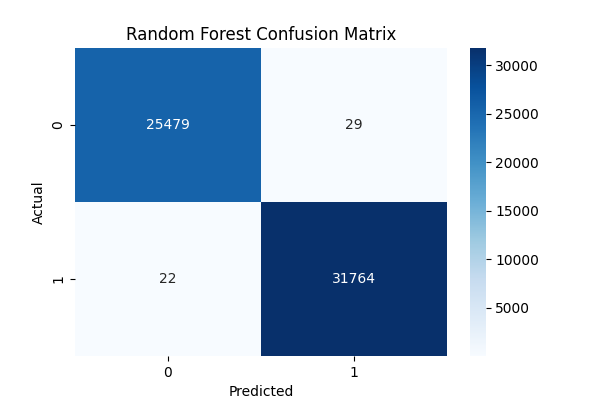
\includegraphics[width=\textwidth]{confusion_matrix_random_forest.png}\caption{Random Forest}\end{subfigure}\hfill
\begin{subfigure}[b]{0.32\textwidth}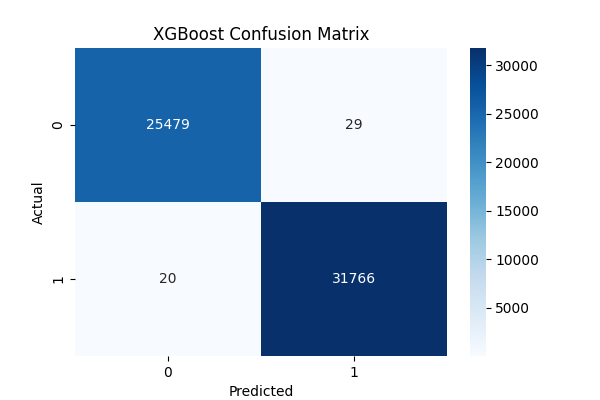
\includegraphics[width=\textwidth]{confusion_matrix_xgboost.png}\caption{XGBoost}\end{subfigure}\hfill
\begin{subfigure}[b]{0.32\textwidth}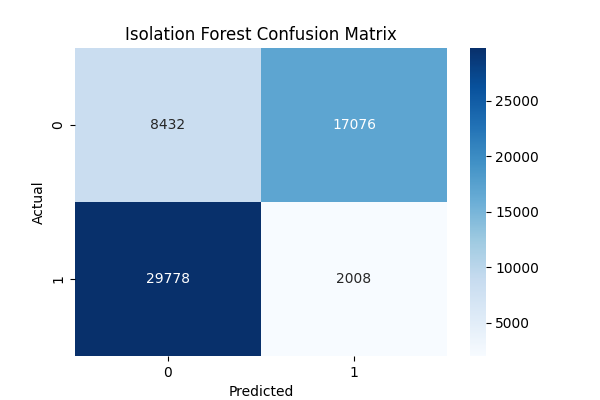
\includegraphics[width=\textwidth]{confusion_matrix_isolation_forest.png}\caption{Isolation Forest}\end{subfigure}
\caption{Confusion matrices of the three models on the test set}
\label{fig:confusion_matrices}
\end{figure}

\begin{figure}[H]
\centering
\begin{subfigure}[b]{0.48\textwidth}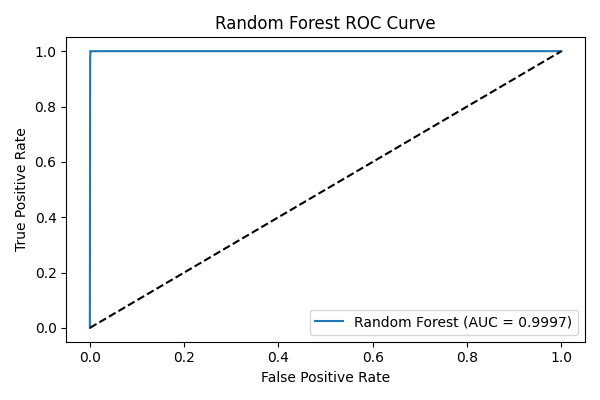
\includegraphics[width=\textwidth]{roc_random_forest.png}\caption{Random Forest}\end{subfigure}\hfill
\begin{subfigure}[b]{0.48\textwidth}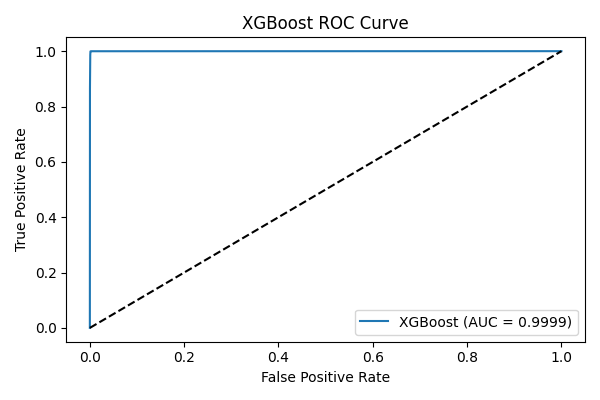
\includegraphics[width=\textwidth]{roc_xgboost.png}\caption{XGBoost}\end{subfigure}
\caption{ROC curves of the supervised models (Random Forest and XGBoost)}
\label{fig:roc_curves}
\end{figure}

\subsubsection{Success Criteria Verification}

The project's final plan defines three performance thresholds that the detection system must achieve. The table below compares the obtained results against these criteria:

\begin{table}[H]
\centering
\caption{Verification of project success criteria}
\label{tab:success}
\begin{tabular}{lccccc}
\toprule
\textbf{Criterion} & \textbf{Threshold} & \textbf{RF} & \textbf{Status} & \textbf{XGBoost} & \textbf{Status} \\
\midrule
F1-Score & $\geq$ 88\% & 99.92\% & \textbf{PASS} & 99.92\% & \textbf{PASS} \\
Accuracy & $\geq$ 90\% & 99.91\% & \textbf{PASS} & 99.91\% & \textbf{PASS} \\
FPR & $<$ 6\% & 0.11\% & \textbf{PASS} & 0.11\% & \textbf{PASS} \\
\bottomrule
\end{tabular}
\end{table}

\noindent Both supervised models (Random Forest and XGBoost) significantly exceed all defined success criteria.

\subsubsection{Analysis of Isolation Forest's Failure}

Isolation Forest was integrated into the architecture for its theoretical capacity to detect stealthy \textbf{"Low and Slow"} attacks. However, empirical results on the CICIDS2017 dataset reveal very poor performance (F1-Score of 7.89\%, FPR of 66.94\%). This underperformance is explained by two fundamental factors:

\paragraph{1. The Majority Anomaly Paradox:} Isolation Forest is mathematically designed to isolate data points that are \textit{"few and different"}, i.e., anomalies typically representing less than 5\% of the dataset. However, in our CICIDS2017 dataset, the \texttt{PortScan} class constitutes \textbf{55.48\%} of the traffic — it is the \textit{majority} class. The algorithm, trained on the complete set (normal traffic + attacks), is unable to distinguish attacks as anomalies since they represent the statistical norm of the dataset.

\paragraph{2. Mismatch between Aggressive and Stealthy Signatures:} The port scans present in the CICIDS2017 dataset are primarily aggressive \texttt{Nmap} scans, generating a massive burst volume of packets. These signatures are dense and do not match the "Low and Slow" profile (spaced flows over time, low volume) for which Isolation Forest was selected.

\paragraph{Conclusion:} This failure does not undermine the architectural relevance of Isolation Forest in the AEGIS Entropy system. Instead, it demonstrates a methodological limitation: to be effective in anomaly detection, Isolation Forest must be trained exclusively on verified \textbf{BENIGN} traffic (semi-supervised approach) in order to establish a clean baseline of normal network behavior. In a production environment where attacks are genuinely rare and stealthy, this model would regain its relevance. For detecting the aggressive scans present in this dataset, the supervised models (Random Forest and XGBoost) are vastly superior.

%% =============================================================
\subsection{Conclusion}

This chapter presented the complete design and implementation of the machine learning detection pipeline for the AEGIS Entropy system. The pipeline, built according to a rigorous methodology, includes:

\begin{enumerate}
    \item \textbf{Comprehensive data preprocessing} (cleaning, IQR outlier detection, skewness correction via logarithmic transformation)
    \item \textbf{Normalization} via StandardScaler with strict data leakage prevention
    \item \textbf{Class balancing} via SMOTE applied solely on the training set
    \item The \textbf{training} of three complementary models (Random Forest, XGBoost, Isolation Forest)
    \item A \textbf{10-fold Stratified Cross-Validation} confirming the stability of results
    \item A comprehensive \textbf{evaluation} using six metrics and verification of success criteria
\end{enumerate}

The results demonstrate that the supervised models achieve exceptional performance: an F1-Score of \textbf{99.92\%}, an Accuracy of \textbf{99.91\%}, and an FPR of only \textbf{0.11\%}, vastly exceeding the thresholds required by the project's final plan. The analysis of Isolation Forest identified the necessary conditions for its effective deployment in a real-world environment.

The pipeline is now ready for integration with the real-time capture modules, the honeypot system, and the monitoring dashboard, which will be the subjects of the subsequent chapters.

% Note: ml_pipeline_report_part2.tex must be in the same report/ directory

\end{document}
